\section{Supplementary material}

\subsection{Reproducibility statement}

The v3 workspace is a zero-new-inference reanalysis. It reads an existing merged run manifest, resolves raw exact-option cache bundles by cache key, computes the corrected persistence metrics, and generates all paper numbers, figures, and tables from those derived outputs.

\subsection*{Ethics statement}

This study analyzes public benchmark questions with open-weight language models and reports observational statistics over existing cached outputs. The main risk is interpretive overreach. The manuscript mitigates that risk by keeping the claim tied to exact-option score dynamics in the tested panel and by avoiding mechanism claims.

\subsection*{AI-use disclosure}

AI-use disclosure. The authors used AI-assisted tools during the project lifecycle: ChatGPT for brainstorming and experimental design iteration, Codex for implementation assistance, and Claude Opus for drafting and formatting portions of the manuscript and LaTeX source. All scientific decisions, experiments, analyses, code review, result verification, and final manuscript editing were performed and approved by the human authors, who take full responsibility for the paper’s contents.

\subsection{Model summary table}

\begin{center}
\small
\begin{tabular}{@{}lcccc@{}}
\toprule
Model & Med. $\Delta_{250}$ & CI low & CI high & Med. write after $d_2$ \\
\midrule
Qwen 2.5 1.5B & 0.15 & 0.15 & 0.19 & 49\% \\
Qwen 2.5 3B & 0.09 & 0.09 & 0.11 & 38\% \\
Qwen 2.5 7B & 0.15 & 0.15 & 0.15 & 49\% \\
Gemma 2 2B & 0.16 & 0.12 & 0.20 & 61\% \\
Gemma 2 9B & 0.15 & 0.12 & 0.17 & 69\% \\
Gemma 2 27B & 0.13 & 0.11 & 0.16 & 59\% \\
Llama 3.2 1B & 0.13 & 0.13 & 0.20 & 49\% \\
Llama 3.2 3B & 0.19 & 0.15 & 0.19 & 44\% \\
Llama 3.1 8B & 0.16 & 0.13 & 0.19 & 44\% \\
\bottomrule
\end{tabular}

\captionof{table}{\textbf{Descriptive model summary.} The appendix reports model-level medians and confidence intervals for $\Delta_{250}$ together with the median write share after $d_2$.}
\end{center}

\begin{figure}[h]
\centering
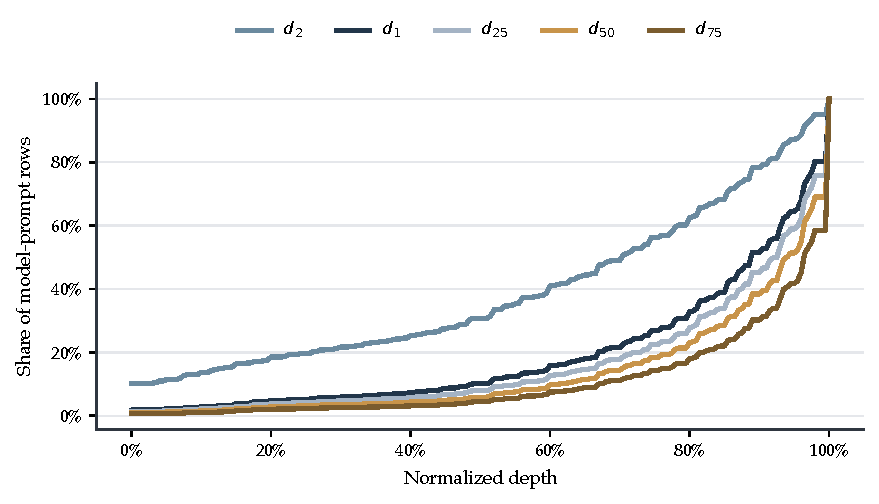
\includegraphics[width=\linewidth]{appendix_pooled_depths.pdf}
\caption{\textbf{Pooled CDFs including the appendix thresholds $d_{25}$ and $d_{75}$.} The same ordering remains visible when the margin threshold is relaxed or tightened.}
\end{figure}

\begin{figure}[h]
\centering
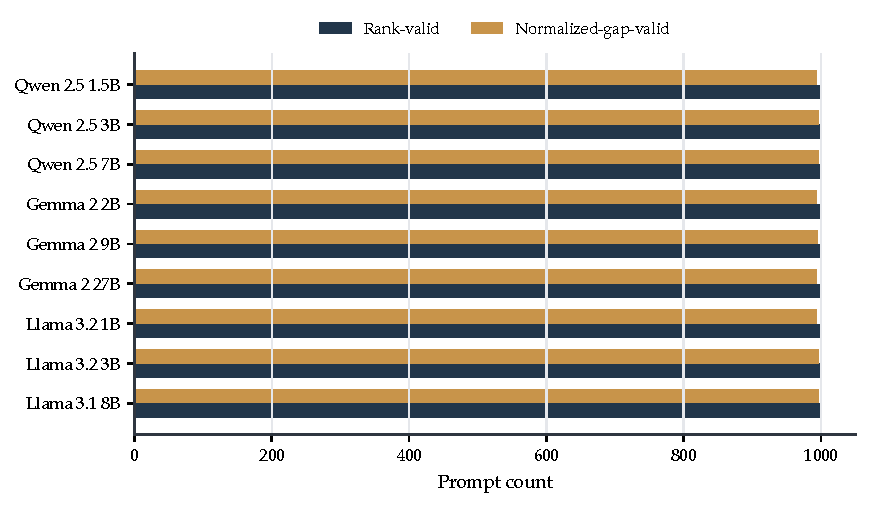
\includegraphics[width=0.92\linewidth]{appendix_valid_counts_by_model.pdf}
\caption{\textbf{Valid prompt counts by model.} Rank-based depths are available for all model-prompt rows. Normalized-gap analyses exclude only cases with a non-positive final gap.}
\end{figure}
